%\documentclass[pdftex,12pt,a4paper]{article}
\documentclass[10pt]{article}

\usepackage[left=2.5cm,top=2.5cm,bottom=2.5cm,right=2.5cm]{geometry}


\usepackage[utf8]{inputenc}
%\usepackage[T1]{fontenc}
\usepackage[spanish]{babel}
\usepackage{amssymb,amsmath,amsthm}
\usepackage{fancyhdr}
\usepackage{bm}
\usepackage{graphics}
\usepackage{graphicx}
\usepackage{caption}
\usepackage{subfig}
\usepackage{setspace}

%%para ecuaciones$$$
\usepackage{listings}

\lstdefinestyle{PY}{
language = Python,
frame = single,
keywordstyle = \color{blue},
commentstyle=\color{red},
basicstyle = \footnotesize \ttfamily,
breaklines=true,
showstringspaces=false            % importante para python
}

\lstdefinestyle{as}{
language = Python,
keywordstyle = \color{blue},
commentstyle=\color{red},
basicstyle = \footnotesize \ttfamily,
breaklines=true,
showstringspaces=false            % importante para python
}
%%%%%%%%%%%%%%%%%%%%%%%%


\usepackage{tikz}
\def\checkmark{\tikz\fill[scale=0.4](0,.35) -- (.25,0) -- (1,.7) -- (.25,.15) -- cycle;}



\newcommand{\HRule}{\rule{\linewidth}{0.25mm}}
\newcommand{\floor}[1]{\lfloor #1 \rfloor}



%%%%%%%%comienza documento%%%%%%%%%%
\begin{document}

%%%%%%%%PORTADA%%%%%
\begin{center}

\includegraphics[width=0.2\textwidth]{images/logo_usm}~\\[1.2cm]
~\\[-1.5cm]

\textsc{\large Universidad T\'ecnica Federico Santa Mar\'ia}\\[0.2cm]
\textsc{\large Departamento de Inform\'atica}\\[0.2cm]
\textit{1er Semestre 2016}\\[4cm]

\HRule \\[0.6cm]
{\Large \textsc{Homework I - Machine Learning - INF}}\\[0.4cm]
{\Large \textit{Prof. }\\[0.1cm]
\HRule \\[0.8cm]

% Author and supervisor
\begin{minipage}{0.4\textwidth}
\begin{center}
\emph{Autor:}\\
Francisco Mena Toro\\ \textit{francisco.mena.13@sansano.usm.cl} \\ 201373504-5 \\
\emph{San Joaqu\'in}
\end{center}
\end{minipage}
\begin{minipage}{0.4\textwidth}
\begin{center}
\emph{Autor:}\\
Francisco Perez Casto\\ \textit{francisco.perezca.13@sansano.usm.cl} \\ 201373516-9 \\
\emph{San Joaqu\'in}
\end{center}
\end{minipage}
}\end{center}

\vspace{2cm}

\newpage


\section{Introducción}
a\\

\section{Supuestos}

a\\

\section{Desarrollo}
Se trabajará sobre datos utilizando regresión lineal para predecir valores...

\subsection{Regresión Lineal Ordinaria (LSS)}

En esta sección se trabaja con un dataset (\textit{prostate-cancer}), donde con determinadas variables, se intentará predecir datos futuros mediante un algoritmo que ajusta con regresión lineal.

\begin{itemize}
\item[a)] Acá se crea el dataset de trabajo, donde en la línea 5 elimina una columna innecesaria, la cual se llama ''\textit{Unnamed: 0}'' que entrega la información de enumeración de los datos, la cual viene por defecto en el dataframe $df$ por lo que no es necesario, es por esto que se elimina con la acción $drop$. Para el caso de la linea 9, elimina la columna llamada ''\textit{train}'' la cual fue extraida y guardada en otra variable anteriormente, además de que no forma parte de las variables del dataset o del target, ya que simboliza un valor de True o False si cada dato corresponde al training set o no.

\item[b)] El dataset se conforma de 97 entradas en el input space ($\chi$), con 9 columnas, de las cuales 8 de estas conforman a las características de estudio las cuales predicirán la novena columna (target). Dentro de los valores del dataset existen valores decimales y valores enteros. Existen características que tienen una escala muy diferente a las otras, tales como la edad (age), la cual tiene una media aritémica muy distintante a las demás características en el dataset. Por otro lado, existen características que poseen una desviación estandar muy alta comparado con el resto, tal como el porcentaje de Gleason escalado 4 o 5 (pgg45).

\item[c)] Es importante normalizar el dataset, así tener una desviación estándar mas estandarizada y no con valores tan alejados entre sí como es el caso del porcentaje de Gleason (pgg45), o con la edad (age)... explicar mas buscar en libros o k se yo.
Resulta conveniente realizar esta operación ya que así se puede realizar un mejor ajuste  sobre los datos, gracias a escalar la data.

\item[d)] Luego se realiza un ajuste lineal por mínimos cuadrados. Donde el argumento de la función que implementa esta regresión lineal es \textit{fit-intercept}, donde no será usado el intercepto en los cálculos ya que los datos ya están normalizados.

\item[e)]Construya una tabla con los pesos y Z-score correspondientes a cada predictor (variable). ¿Que variables estan mas correlacionadas con la respuesta? Si us aramos un nivel de significacionn del 5\%, ¿Para que variables no existe suficiente evidencia que demuestre la relacion con la respuesta?

\begin{table}
  \begin{center}
    \begin{tabular}{|c|c|c|c|} \hline
    Atributo & Coeficiente & Std. Error & Z-score \\ \hline
    Lcavol' &'0.5966394' &'0.1215977' &'4.9066641 \\
 	Lweight' & '0.2723253' &'0.0918286'& '2.9655804 \\
 	Age' & '-0.145638' &'0.0973158' &'-1.496554 \\
 	Lbph' & '0.1892731' & '0.0981576'& '1.9282562 \\
 	Svi' & '0.1794042' & '0.1186893' &'1.5115442 \\
 	Lcp' & '-0.159118' & '0.1483895' &'-1.072302 \\
 	Gleason' & '0.1007800' &'0.1394762'& '0.7225607 \\
 	Pgg45' & '0.1148827'& '0.1475101' &'0.7788125 \\
 	Intercept' & '2.4000628'& '0.0862118'& '27.839132 \\ \hline
    \end{tabular}
  \end{center}
\end{table}


\item[f)] Se estima el error del método regresión lineal ordinario por mínimos cuadrados, donde se tiene data de test ''real'' la cual entrega un error real con el modelo de regresión lineal ordinaria de 0.521274...
Con K = 10 el error de prueba (cross-validation) 0.757237... analizar esto
Con K = 5 el error de prueba es 0.956514... analizar esto

error porcentual de K =10 y K = 5
32.6986805041
46.72001931

Cross-validation presenta un error mas grande que el error ''real'', por lo que esto nos dice que para este caso cross-validation no acierta en la predicción del error. Esto puede deberse principalmente a que la cantidad de datos es bastante poca, por lo que dividir la data en 10 o 5 \textit{folds} no es una operación tan significativa.

\item[j)] Asumir normalidad esta mal por el grafico

\begin{figure}[h]
    \centering
    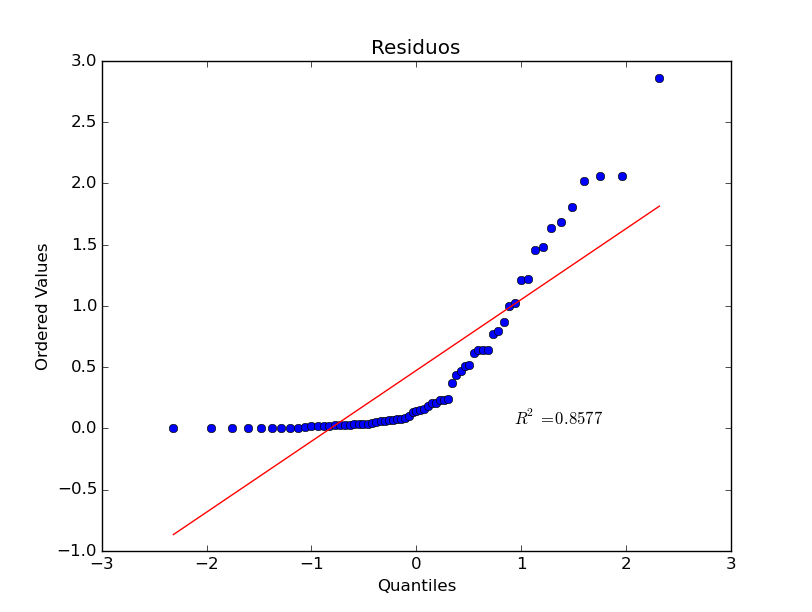
\includegraphics[width=0.55\textwidth]{images/qqplot}
    \caption{Q-Q plot del error de los datos de entrenamiento}
    \label{fig:mesh1}
\end{figure}

A normal Q–Q plot of randomly generated, independent standard exponential data, (X ~ Exp(1)). This Q–Q plot compares a sample of data on the vertical axis to a statistical population on the horizontal axis. The points follow a strongly nonlinear pattern, suggesting that the data are not distributed as a standard normal (X ~ N(0,1)). The offset between the line and the points suggests that the mean of the data is not 0. The median of the points can be determined to be near 0.7

\end{itemize}

\subsection{Selección de Atributos}
Utilizando el mismo dataset (\textit{prostate-cancer}) se realiza un estudio sobre seleccionar los atributos/características escenciales, es decir, que afecten mas el resultado de la variable que se desea predecir (target). Se realizan dos métodos para analizar el impacto que tiene cada atributo sobre el target, una es mediante FSS en donde se va seleccionando cada atributo, uno por uno, siendo esa variable la mejor en ese momento. Otra es mediante BSS, la cual va elimimando un atributo en cada iteración, siendo ese atributo el que menos influencia tiene en el resultado de la variable target.

\begin{itemize}
\item[a)] FSS parte de un modelo sin atributos (variables) y agrega uno a la vez, eligiendo la mejor localmente. Para este caso la selección fue en el orden siguiente:

selected = Lcavol ...
totalvars=2, mse = 0.876172
selected = Lweight ...
totalvars=3, mse = 0.752606
selected = Lbph ...
totalvars=4, mse = 0.748883
selected = Svi ...
totalvars=5, mse = 0.746635
selected = Pgg45 ...
totalvars=6, mse = 0.748007
selected = Lcp ...
totalvars=7, mse = 0.734094
selected = Age ...
totalvars=8, mse = 0.726706
selected = Gleason ...
totalvars=9, mse = 0.757237

Donde se puede ver como la primera característica en escoger es \textit{Lcavol}, y la última es \textit{Gleason}.

\begin{figure}[h]
    \centering
    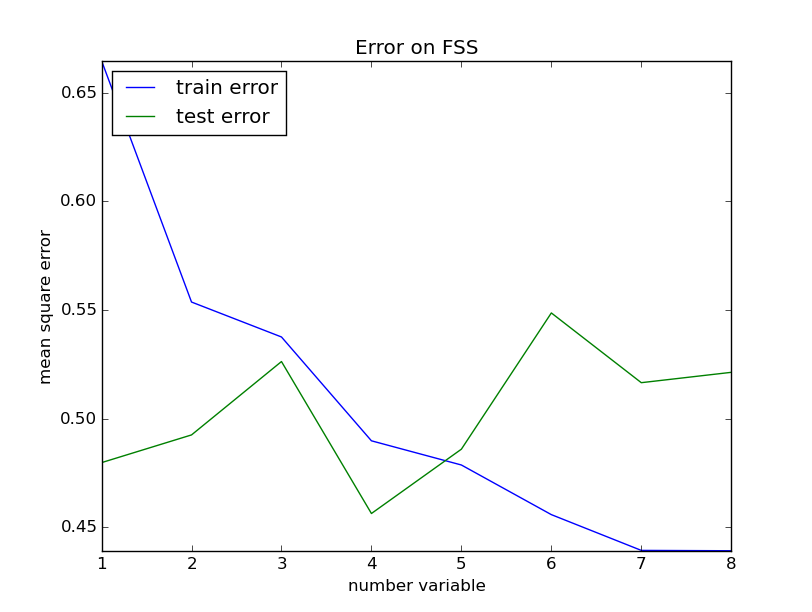
\includegraphics[width=0.55\textwidth]{images/fss}
    \caption{errores en FSS en regresión lineal ordinaria}
    \label{fig:mesh1}
\end{figure}


\item[b)] BSS parte de un modelo completo (todas las características), eliminando una característica a la vez. Para este caso, el orden de eliminar cada atributo fue el siguiente:

selected to delete = Gleason ...
totalvars=8, mse = 0.726706
selected to delete = Age ...
totalvars=7, mse = 0.734094
selected to delete = Lcp ...
totalvars=6, mse = 0.748007
selected to delete = Pgg45 ...
totalvars=5, mse = 0.746635
selected to delete = Svi ...
totalvars=4, mse = 0.748883
selected to delete = Lbph ...
totalvars=3, mse = 0.752606
selected to delete = Lweight ...
totalvars=2, mse = 0.876172
selected to delete = Lcavol ...
totalvars=1, mse = 1.795596

Donde se puede ver como la primera variable en ser eliminada fue la característica \textit{Gleason} y la última en ser eliminada fue \textit{Lcavol}.

\begin{figure}[h]
    \centering
    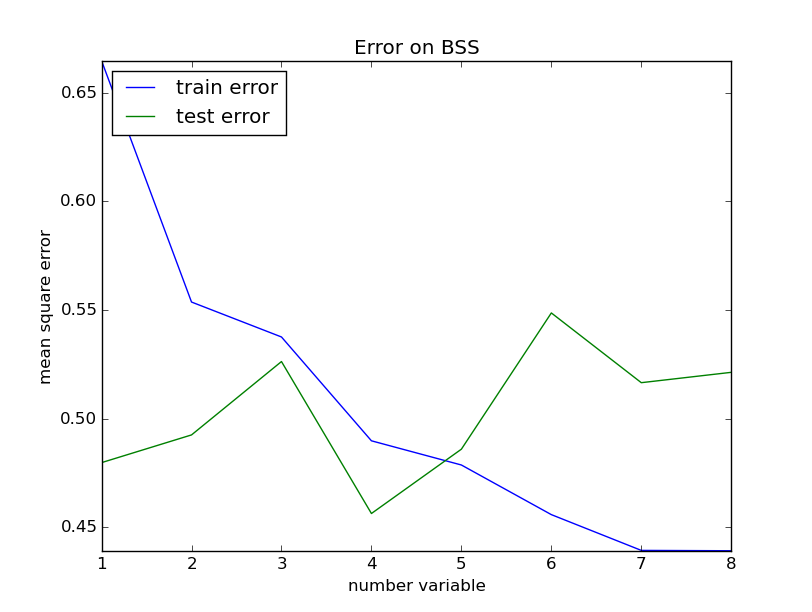
\includegraphics[width=0.55\textwidth]{images/bss}
    \caption{error BSS en regresión lineal ordinaria}
    \label{fig:mesh1}
\end{figure}
\end{itemize}

\subsection{Regularización}

En esta parte del informe se tratara el tema de la regularización, en donde se castigan los coeficientes altos del modelo lineal, regularizando estos y dandoles un límite de valor para tomar y ver como afecta esto al modelo. Para eso se harán distintas comparaciones entre los errores de test y entrenamiento, para distintos algoritmos de aprendizaje dodne cada uno tiene un método de regularización diferente, incluyendo diferentes rangos en la regularización.
 
\begin{itemize}

\item[a)] Se utiliza el método de ''\textit{Ridge Regression}'' el cual regulariza los atributos para obtener una modelo lineal mas preciso para la data futura.\\
En el código entregado, en la tercera línea se elimina la columna "intercept", puesto que ya no se necesita, ya que la regularización es sobre los atributos/características del modelo, por lo que el intercepto no es modificado. En la novena línea se ejecuta el método de Ridge a través de factorización svd, con el parametro \textit{fit intercept} asignado como \textit{True}, puesto que como la columna fue eliminada, el mismo método se encarga de calcular el intercepto.

 Se puede observar del grafico que las caracteristicas que poseen mas peso son Lcavol, Lweight y svi
 Esto apoya las afirmaciones anteriores de los metodos FSS y BSS.

\item[b)] Para este caso se utiliza el método de ''\textit{Lasso}'', el cual regulariza los atributos de una manera mas estricta que ''\textit{Ridge}'', por lo que tiene una penalización mas alta para los atributos, siendo más riguroso que Ridge al decir cual característica tendrá mas peso en el modelo.

explicar
\item[c)] Para este caso se ve como afecta la penalización de la variable \textit{alpha} para los distintos atributos, viendo el error de test y entrenamiento en función de los distintos alphas seleccionados en un rango dado, mostrando a continuación:\\

 Al analizar el grafico de los errores de test y entrenamiento en funcion de los alpha, se puede
 visualizar que el error de entrenamiento a medida que disminuye el valor de alpha, se observa que
 baja su valor, lo cual es esperado puesto que son los datos con los que se entreno el algoritmo.
 Tambien es esperado que el error de test empiece a ser mas alto que el de entrenamiento despues
 de cierto punto. Es importante notar que ambos errores empiezan a tener un valor constante
 despues de los valores de alpha 10e-1 y 10e-2.

\item[d)] Analogo al caso anterior, se ve como afecta la penalización de la variable \textit{alpha} para los distintos atributos:\\


\item[e)] Para conocer qué valor es el óptimo para \textit{alpha}, se utiliza \textit{cross-validation}, probando distintos alphas y midiendo el error con los \textit{k-folds} y determinando cual alpha es el óptimo para cada modelo de regresión lineal (Ridge y Lasso).

\end{itemize}




 
\section{Anexo}

%\lstinputlisting[style = as]{codigos/acp.py}

Lo demás adjuntado en archivos .py

\section{Bibliografía}
\begin{itemize}
\item \begin{verbatim}
Hastie, T.; Tibshirani, R., Friedman, J. (2009), The Elements of Statistical Learning, Second Edition.
Springer New York Inc.
\end{verbatim}
\end{itemize}
\end{document}
